%% ============================================
%% ================ Preambule =================
%% ============================================
\documentclass[]{scrartcl}
\usepackage[margin = 0.5in]{geometry}

\usepackage[pdftex,unicode, 
colorlinks=true,
linkcolor = blue]{hyperref}	% нумерование страниц, ссылки!!!!ИМЕННО В ТАКОМ ПОРЯДКЕ СО СЛЕДУЮЩИМ ПАКЕТОМ
%\usepackage[warn]{mathtext}				% Поддержка русского текста в формулах
\usepackage[T1, T2A]{fontenc}			% Пакет выбора кодировки и шрифтов
\usepackage[utf8]{inputenc} 			% любая желаемая кодировка
\usepackage[english]{babel}		% поддержка русского языка
\usepackage{wrapfig}					% Плавающие картинки
\usepackage{amssymb, amsmath}			% стилевой пакет для формул
\usepackage{algorithm}
\usepackage{algorithmic} 


\ifpdf
\usepackage{cmap} 				% чтобы работал поиск по PDF
\usepackage[pdftex]{graphicx}
%\usepackage{pgfplotstable}		% Для вставки таблиц.
\pdfcompresslevel=9 			% сжимать PDF
\else
\usepackage{graphicx}
\fi

\graphicspath{{./figures/}}
\usepackage{subcaption}
%% ============================================
%% ================ Info =================
%% ============================================
\title{Использование тензорных сетей для сжатия и восстановления изображений}
\author{\begin{tabular}{c c}
	  	 Александр Моложавенко &  molozhavenko.aa@phystech.edu\\
		\end{tabular}}
\date{Project Proposal}

\begin{document}

\maketitle

\begin{abstract}
В этом проекте рассматривается возможность использования тензорных сетей для задач восстановления изображения по значениям в небольшом числе пикселей (tensor completion), а также для сжатия изображений. 
\end{abstract}

\section{Идея}
    
    С помощью тензорных сетей (\textit{PEPS}, \textit{Tensor Ring}, \textit{Tensor Train}),  алгоритма \textit{Greedy-TN} \cite{DBLP:journals/corr/abs-2008-05437}, его модифи-каций и алгоритмами \textit{HOSVD, ALS} найти оптимальные конфигурации для минимально возможного по количеству параметров представления изображений. Аналогично этими методами решается задача восста-новления изображений.
    
\subsection{Проблема}
    
    Пусть имеется картинка $M \in \mathbb{R}^{3 \times d_w \times d_h}$, задаваемая тремя матрицами пикселей (фильтр синего, фильтр красного и фильтр зеленого) или трехмерным тензором.Преобразуем трёхиндексную матрицу $M$ в много индексную матрицу (в тензор высокого порядка) по основанию $b$, то есть:

$$
M \in \mathbb{R}^{3 \times d_w \times d_h} \mapsto \mathcal{T} \in \mathbb{R}^{b \times b \times \dots \times b}.
$$


    Количество мод полученного тензора, равняется $N = \log_b (3\cdot d_h \cdot d_w)$. Количество элементов в таком представлении изображение есть $3 \cdot d_w \cdot d_h = b ^ N$. Однако, если к полученному тензору высокого порядка применить \textit{Tensor Train Decomposition} из $N$ тензоров свертке с максимальном рангом тензорного поезда $m$, то придется хранить всего лишь около $N\cdot b \cdot m^2$ элементов. Что при правильной оптимизации ранга разлажения может дать существенное сжатие.

В терминах статьи  \cite{DBLP:journals/corr/abs-2008-05437} введем в рассмотрение тензорную сеть $\text{TN}(\mathcal{G}^{(1)}, \mathcal{G}^{(2)}, \dots, \mathcal{G}^{(N)})$, которая в свертке по заданным в ней модам даёт тензор $\mathcal{W} \in \mathbb{R}^{b \times b \times \dots \times b}$. В этих обозначениях проблемы восстановления и сжатия изображений перепишутся следующим образом:

\subsubsection{Image compression}
\begin{equation}\label{ImComprProbStatement}
\|\mathcal{T} - \text{TN}(\mathcal{G}^{(1)}, \mathcal{G}^{(2)}, \dots, \mathcal{G}^{(N)})\|_F^2 \to \min\limits_{\mathcal{G}^{(1)}, \mathcal{G}^{(2)}, \dots, \mathcal{G}^{(N)}},
\end{equation}


причём в зависимости от выбранного метода оптимизации данной функции будут или не будут наклады-ваться дополнительные условия связи между \textit{core}-тензорами тензорной сети (адаптивный метод \textit{Greedy-TN}, например автоматически подбирает нужные связи)

\subsubsection{Image Completion}
\begin{equation}\label{ImComplProbStatement}
\frac{1}{|\Omega|}\sum\limits_{(i_1, \dots, i_N) \in \Omega}\left(\mathcal{T}_{i_1, \dots, i_N} - \text{TN}(\mathcal{G}^{(1)}, \mathcal{G}^{(2)}, \dots, \mathcal{G}^{(N)})_{i_1, \dots, i_N}\right)^2 \to \min\limits_{\mathcal{G}^{(1)}, \mathcal{G}^{(2)}, \dots, \mathcal{G}^{(N)}},
\end{equation}

где $\Omega$ -- множество индексов, значения под которыми нам известны (индексы известных частей картинки после её отображения в тензор высокого порядка).

\newpage
\section{Литературный обзор}
\documentclass{beamer}
\beamertemplatenavigationsymbolsempty
\setbeamertemplate{blocks}[rounded=true, shadow=true]
\setbeamertemplate{footline}[page number]
\usepackage[english,russian]{babel}
\usepackage[utf8]{inputenc}
\usepackage[english]{babel}
\usepackage{amssymb,amsfonts,amsmath,mathtext}
\usepackage{subfig}
\usepackage[all]{xy} % xy package for diagrams
\usepackage{array}
\usepackage{multicol}% many columns in slide
\usepackage{hyperref}% urls
\usepackage{hhline}%tables
\usepackage{babel,blindtext}
% Your figures are here:
\graphicspath{ {fig/} {../fig/} }

%----------------------------------------------------------------------------------------------------------
\title[\hbox to 56mm]{Solution of a block multidimensional eigenvalues search problem}
\author[~Molozhavenko]{Автор: Моложавенко А.А. \\ Научный руководитель: Гасников А.В. \\ Научный консультант: Рахуба М.В.}
\institute{Московский физико-технический институт\\ Физтех-школа прикладной математики и информатики\\Кафедра Интеллектуальные системы}


%----------------------------------------------------------------------------------------------------------
\begin{document}
%----------------------------------------------------------------------------------------------------------
\begin{frame}
\thispagestyle{empty}
\maketitle
\end{frame}
%-----------------------------------------------------------------------------------------------------
%\begin{frame}{Goal of research}
%..
%\end{frame}
%-----------------------------------------------------------------------------------------------------
\begin{frame}{Что уже было сделано?}

\begin{itemize}
    \item Знакомство с основными тензорными разложениями (TT, TR, Tucker)
    \item Разобрана статья \cite{DBLP:journals/corr/abs-2008-05437} о тензорных сетях и алгоритмах на них
    \item Проведены численные эксперименты восстановления и сжатия изображений с помощью тензорных сетей
    
\end{itemize}
    
\end{frame}

\begin{frame}{Какие были получены результаты?}
    
    \begin{columns}
        \begin{column}{0.245\textwidth}
            \begin{figure}
                \centering
                    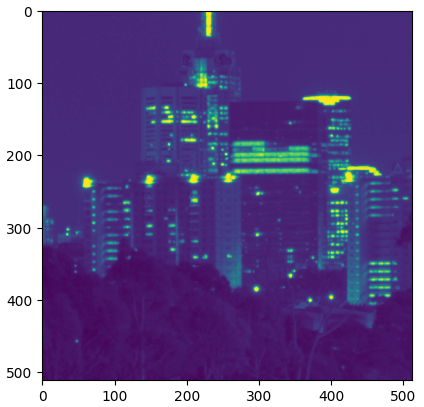
\includegraphics[width=\linewidth]{init.PNG}
                    \caption{Исходное изображение}\label{fig:awesome_image1}
            \end{figure}
        \end{column}
        \begin{column}{0.245\textwidth}
            \begin{figure}
                \centering
                    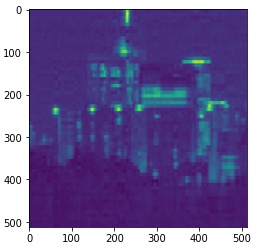
\includegraphics[width=\linewidth]{4.PNG}
                    \caption{96\% сжатие}\label{fig:awesome_image1}
            \end{figure}
        \end{column}
        \begin{column}{0.245\textwidth}
            % \begin{figure}
            %     \centering
            %         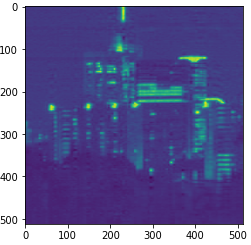
\includegraphics[width=\linewidth]{9.PNG}
            %         \caption{91\% сжатие}\label{fig:awesome_image1}
            % \end{figure}
        \end{column}
        \begin{column}{0.245\textwidth}
            \begin{figure}
                \centering
                    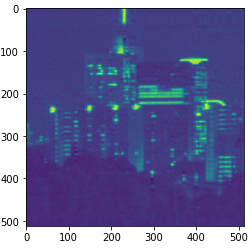
\includegraphics[width=\linewidth]{16.PNG}
                    \caption{84\% сжатие}\label{fig:awesome_image1}
            \end{figure}
        \end{column}
    \end{columns}

\end{frame}

\begin{frame}{Какие были получены результаты?}
    
    \begin{columns}
        \begin{column}{0.47\textwidth}
            \begin{figure}
                \centering
                    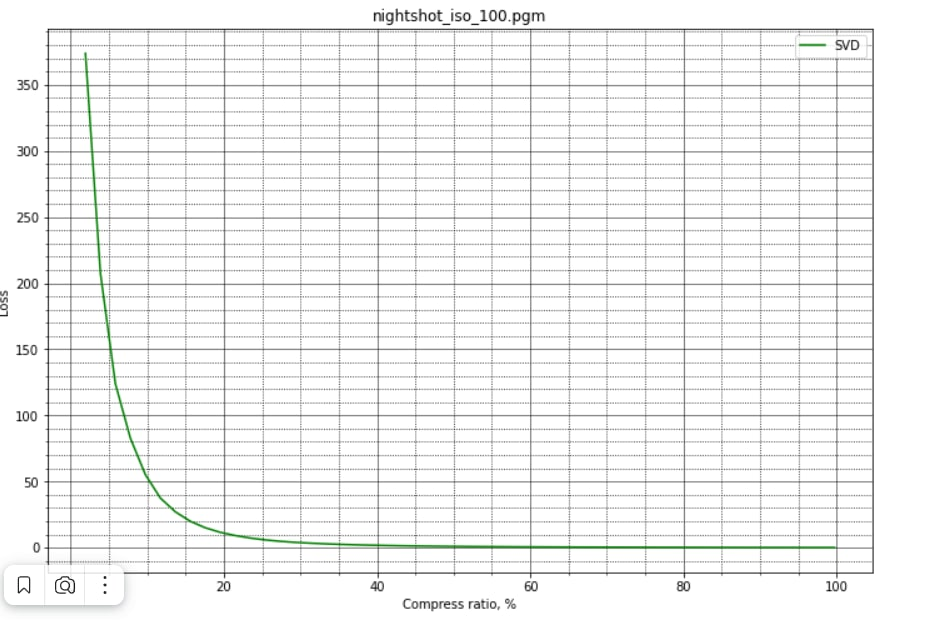
\includegraphics[width=\linewidth]{svd.jpg}
                    \caption{Сжатие SVD}\label{fig:awesome_image1}
            \end{figure}
        \end{column}
        \begin{column}{0.47\textwidth}
            \begin{figure}
                \centering
                    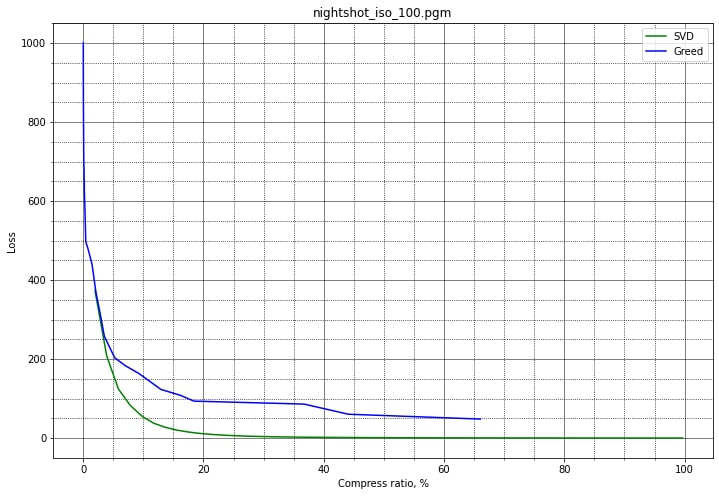
\includegraphics[width=\linewidth]{greed.jpg}
                    \caption{Сжатие алгоритмом из статьи}\label{fig:awesome_image1}
            \end{figure}
        \end{column}
    \end{columns}
        
\end{frame}

\begin{frame}{Что будет дальше?}
\begin{enumerate}
    \item[1)] Освежу в памяти статью \cite{Krumnow2019ComputingEW} 
    \item[2)] Обобщу задачу оптимизации изложенную в статье на тензорные поезда
    \item[3)] Решу полученную задачу
    \item[4)] Проведу численные эксперименты
\end{enumerate}
\end{frame}

\begin{frame}{Источники}
    \bibliographystyle{unsrt}
    \bibliography{biblio}
\end{frame}

\end{document} 

\newpage
\documentclass{beamer}
\beamertemplatenavigationsymbolsempty
\setbeamertemplate{blocks}[rounded=true, shadow=true]
\setbeamertemplate{footline}[page number]
\usepackage[english,russian]{babel}
\usepackage[utf8]{inputenc}
\usepackage[english]{babel}
\usepackage{amssymb,amsfonts,amsmath,mathtext}
\usepackage{subfig}
\usepackage[all]{xy} % xy package for diagrams
\usepackage{array}
\usepackage{multicol}% many columns in slide
\usepackage{hyperref}% urls
\usepackage{hhline}%tables
\usepackage{babel,blindtext}
% Your figures are here:
\graphicspath{ {fig/} {../fig/} }

%----------------------------------------------------------------------------------------------------------
\title[\hbox to 56mm]{Solution of a block multidimensional eigenvalues search problem}
\author[~Molozhavenko]{Автор: Моложавенко А.А. \\ Научный руководитель: Гасников А.В. \\ Научный консультант: Рахуба М.В.}
\institute{Московский физико-технический институт\\ Физтех-школа прикладной математики и информатики\\Кафедра Интеллектуальные системы}


%----------------------------------------------------------------------------------------------------------
\begin{document}
%----------------------------------------------------------------------------------------------------------
\begin{frame}
\thispagestyle{empty}
\maketitle
\end{frame}
%-----------------------------------------------------------------------------------------------------
%\begin{frame}{Goal of research}
%..
%\end{frame}
%-----------------------------------------------------------------------------------------------------
\begin{frame}{Что уже было сделано?}

\begin{itemize}
    \item Знакомство с основными тензорными разложениями (TT, TR, Tucker)
    \item Разобрана статья \cite{DBLP:journals/corr/abs-2008-05437} о тензорных сетях и алгоритмах на них
    \item Проведены численные эксперименты восстановления и сжатия изображений с помощью тензорных сетей
    
\end{itemize}
    
\end{frame}

\begin{frame}{Какие были получены результаты?}
    
    \begin{columns}
        \begin{column}{0.245\textwidth}
            \begin{figure}
                \centering
                    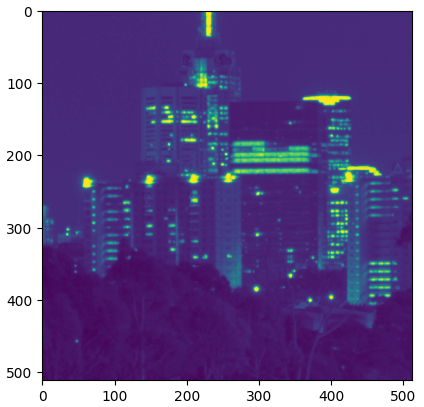
\includegraphics[width=\linewidth]{init.PNG}
                    \caption{Исходное изображение}\label{fig:awesome_image1}
            \end{figure}
        \end{column}
        \begin{column}{0.245\textwidth}
            \begin{figure}
                \centering
                    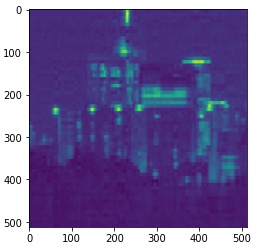
\includegraphics[width=\linewidth]{4.PNG}
                    \caption{96\% сжатие}\label{fig:awesome_image1}
            \end{figure}
        \end{column}
        \begin{column}{0.245\textwidth}
            % \begin{figure}
            %     \centering
            %         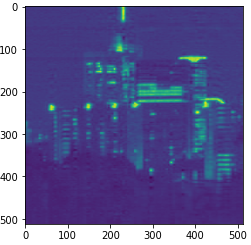
\includegraphics[width=\linewidth]{9.PNG}
            %         \caption{91\% сжатие}\label{fig:awesome_image1}
            % \end{figure}
        \end{column}
        \begin{column}{0.245\textwidth}
            \begin{figure}
                \centering
                    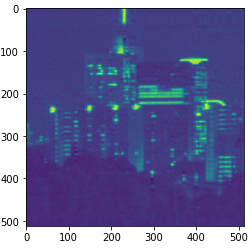
\includegraphics[width=\linewidth]{16.PNG}
                    \caption{84\% сжатие}\label{fig:awesome_image1}
            \end{figure}
        \end{column}
    \end{columns}

\end{frame}

\begin{frame}{Какие были получены результаты?}
    
    \begin{columns}
        \begin{column}{0.47\textwidth}
            \begin{figure}
                \centering
                    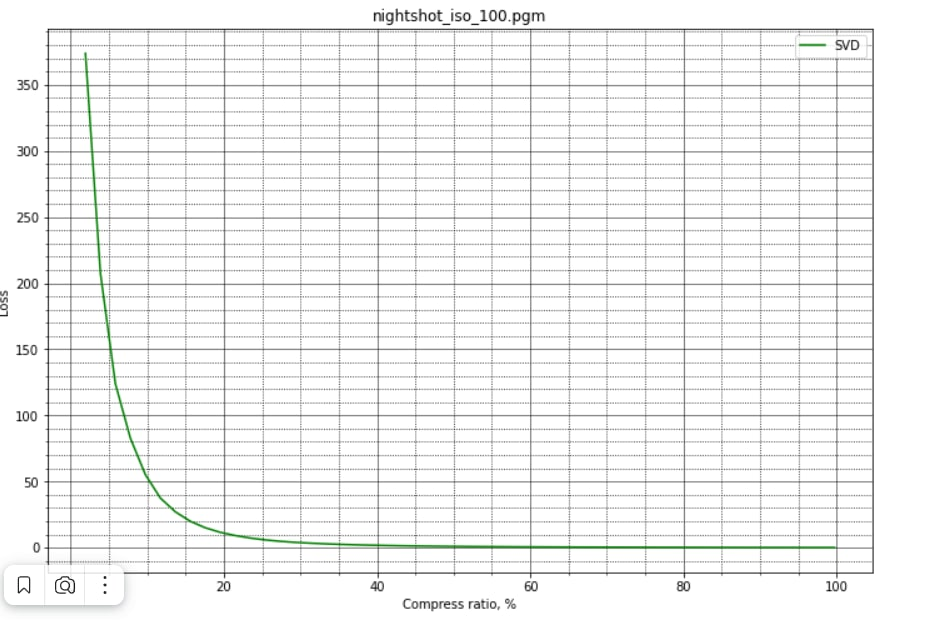
\includegraphics[width=\linewidth]{svd.jpg}
                    \caption{Сжатие SVD}\label{fig:awesome_image1}
            \end{figure}
        \end{column}
        \begin{column}{0.47\textwidth}
            \begin{figure}
                \centering
                    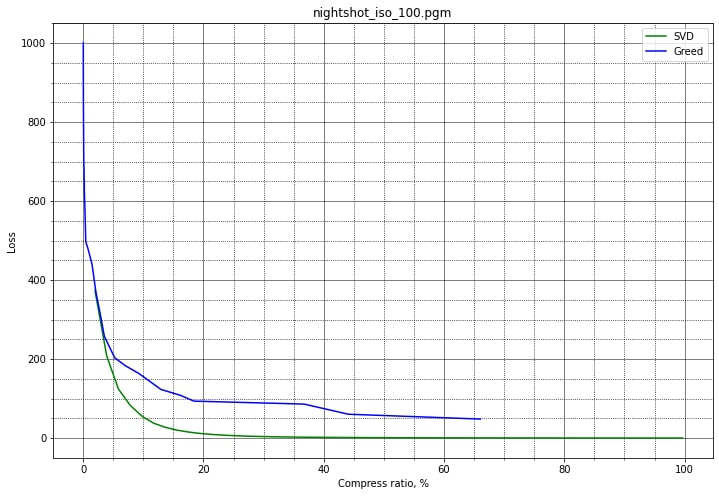
\includegraphics[width=\linewidth]{greed.jpg}
                    \caption{Сжатие алгоритмом из статьи}\label{fig:awesome_image1}
            \end{figure}
        \end{column}
    \end{columns}
        
\end{frame}

\begin{frame}{Что будет дальше?}
\begin{enumerate}
    \item[1)] Освежу в памяти статью \cite{Krumnow2019ComputingEW} 
    \item[2)] Обобщу задачу оптимизации изложенную в статье на тензорные поезда
    \item[3)] Решу полученную задачу
    \item[4)] Проведу численные эксперименты
\end{enumerate}
\end{frame}

\begin{frame}{Источники}
    \bibliographystyle{unsrt}
    \bibliography{biblio}
\end{frame}

\end{document} 

\documentclass{beamer}
\beamertemplatenavigationsymbolsempty
\setbeamertemplate{blocks}[rounded=true, shadow=true]
\setbeamertemplate{footline}[page number]
\usepackage[english,russian]{babel}
\usepackage[utf8]{inputenc}
\usepackage[english]{babel}
\usepackage{amssymb,amsfonts,amsmath,mathtext}
\usepackage{subfig}
\usepackage[all]{xy} % xy package for diagrams
\usepackage{array}
\usepackage{multicol}% many columns in slide
\usepackage{hyperref}% urls
\usepackage{hhline}%tables
\usepackage{babel,blindtext}
% Your figures are here:
\graphicspath{ {fig/} {../fig/} }

%----------------------------------------------------------------------------------------------------------
\title[\hbox to 56mm]{Solution of a block multidimensional eigenvalues search problem}
\author[~Molozhavenko]{Автор: Моложавенко А.А. \\ Научный руководитель: Гасников А.В. \\ Научный консультант: Рахуба М.В.}
\institute{Московский физико-технический институт\\ Физтех-школа прикладной математики и информатики\\Кафедра Интеллектуальные системы}


%----------------------------------------------------------------------------------------------------------
\begin{document}
%----------------------------------------------------------------------------------------------------------
\begin{frame}
\thispagestyle{empty}
\maketitle
\end{frame}
%-----------------------------------------------------------------------------------------------------
%\begin{frame}{Goal of research}
%..
%\end{frame}
%-----------------------------------------------------------------------------------------------------
\begin{frame}{Что уже было сделано?}

\begin{itemize}
    \item Знакомство с основными тензорными разложениями (TT, TR, Tucker)
    \item Разобрана статья \cite{DBLP:journals/corr/abs-2008-05437} о тензорных сетях и алгоритмах на них
    \item Проведены численные эксперименты восстановления и сжатия изображений с помощью тензорных сетей
    
\end{itemize}
    
\end{frame}

\begin{frame}{Какие были получены результаты?}
    
    \begin{columns}
        \begin{column}{0.245\textwidth}
            \begin{figure}
                \centering
                    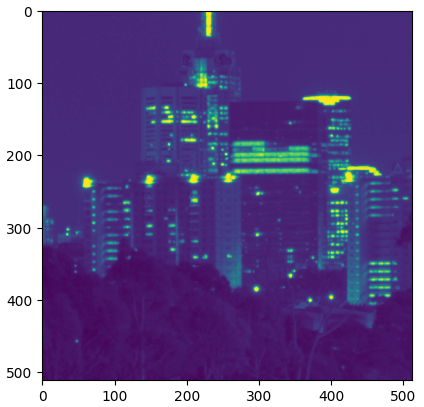
\includegraphics[width=\linewidth]{init.PNG}
                    \caption{Исходное изображение}\label{fig:awesome_image1}
            \end{figure}
        \end{column}
        \begin{column}{0.245\textwidth}
            \begin{figure}
                \centering
                    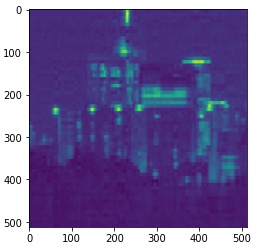
\includegraphics[width=\linewidth]{4.PNG}
                    \caption{96\% сжатие}\label{fig:awesome_image1}
            \end{figure}
        \end{column}
        \begin{column}{0.245\textwidth}
            % \begin{figure}
            %     \centering
            %         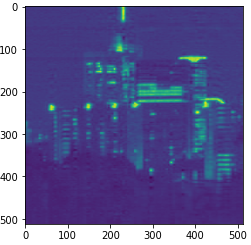
\includegraphics[width=\linewidth]{9.PNG}
            %         \caption{91\% сжатие}\label{fig:awesome_image1}
            % \end{figure}
        \end{column}
        \begin{column}{0.245\textwidth}
            \begin{figure}
                \centering
                    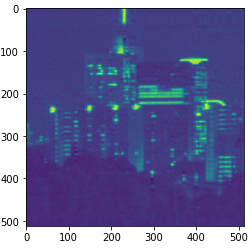
\includegraphics[width=\linewidth]{16.PNG}
                    \caption{84\% сжатие}\label{fig:awesome_image1}
            \end{figure}
        \end{column}
    \end{columns}

\end{frame}

\begin{frame}{Какие были получены результаты?}
    
    \begin{columns}
        \begin{column}{0.47\textwidth}
            \begin{figure}
                \centering
                    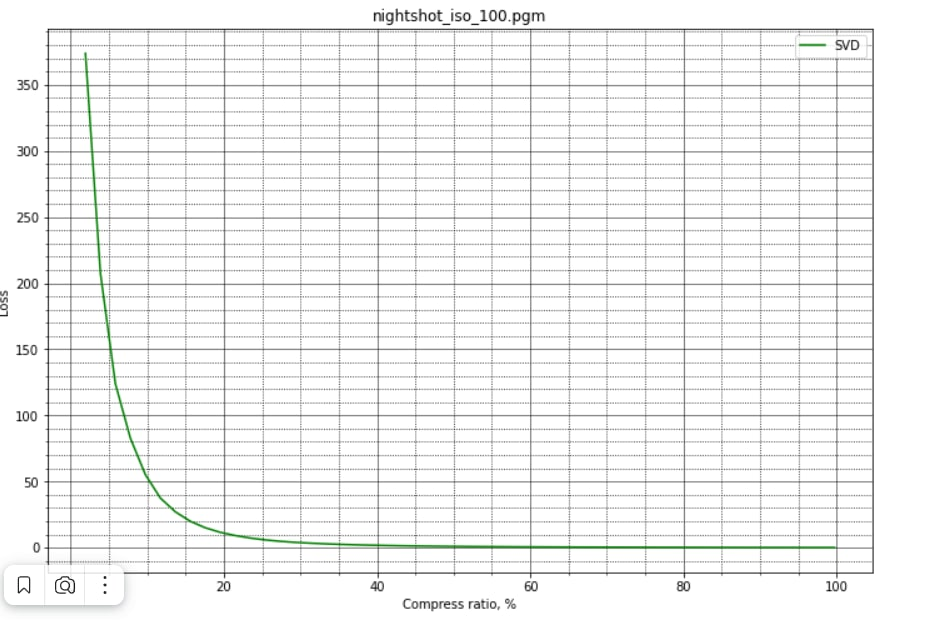
\includegraphics[width=\linewidth]{svd.jpg}
                    \caption{Сжатие SVD}\label{fig:awesome_image1}
            \end{figure}
        \end{column}
        \begin{column}{0.47\textwidth}
            \begin{figure}
                \centering
                    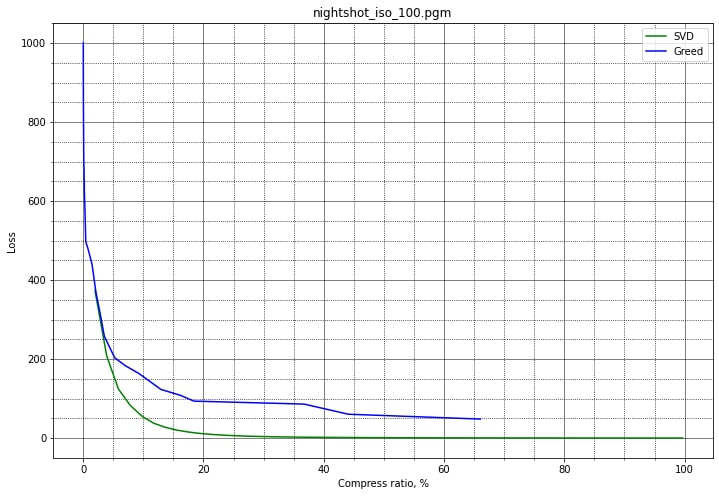
\includegraphics[width=\linewidth]{greed.jpg}
                    \caption{Сжатие алгоритмом из статьи}\label{fig:awesome_image1}
            \end{figure}
        \end{column}
    \end{columns}
        
\end{frame}

\begin{frame}{Что будет дальше?}
\begin{enumerate}
    \item[1)] Освежу в памяти статью \cite{Krumnow2019ComputingEW} 
    \item[2)] Обобщу задачу оптимизации изложенную в статье на тензорные поезда
    \item[3)] Решу полученную задачу
    \item[4)] Проведу численные эксперименты
\end{enumerate}
\end{frame}

\begin{frame}{Источники}
    \bibliographystyle{unsrt}
    \bibliography{biblio}
\end{frame}

\end{document} 

\documentclass{beamer}
\beamertemplatenavigationsymbolsempty
\setbeamertemplate{blocks}[rounded=true, shadow=true]
\setbeamertemplate{footline}[page number]
\usepackage[english,russian]{babel}
\usepackage[utf8]{inputenc}
\usepackage[english]{babel}
\usepackage{amssymb,amsfonts,amsmath,mathtext}
\usepackage{subfig}
\usepackage[all]{xy} % xy package for diagrams
\usepackage{array}
\usepackage{multicol}% many columns in slide
\usepackage{hyperref}% urls
\usepackage{hhline}%tables
\usepackage{babel,blindtext}
% Your figures are here:
\graphicspath{ {fig/} {../fig/} }

%----------------------------------------------------------------------------------------------------------
\title[\hbox to 56mm]{Solution of a block multidimensional eigenvalues search problem}
\author[~Molozhavenko]{Автор: Моложавенко А.А. \\ Научный руководитель: Гасников А.В. \\ Научный консультант: Рахуба М.В.}
\institute{Московский физико-технический институт\\ Физтех-школа прикладной математики и информатики\\Кафедра Интеллектуальные системы}


%----------------------------------------------------------------------------------------------------------
\begin{document}
%----------------------------------------------------------------------------------------------------------
\begin{frame}
\thispagestyle{empty}
\maketitle
\end{frame}
%-----------------------------------------------------------------------------------------------------
%\begin{frame}{Goal of research}
%..
%\end{frame}
%-----------------------------------------------------------------------------------------------------
\begin{frame}{Что уже было сделано?}

\begin{itemize}
    \item Знакомство с основными тензорными разложениями (TT, TR, Tucker)
    \item Разобрана статья \cite{DBLP:journals/corr/abs-2008-05437} о тензорных сетях и алгоритмах на них
    \item Проведены численные эксперименты восстановления и сжатия изображений с помощью тензорных сетей
    
\end{itemize}
    
\end{frame}

\begin{frame}{Какие были получены результаты?}
    
    \begin{columns}
        \begin{column}{0.245\textwidth}
            \begin{figure}
                \centering
                    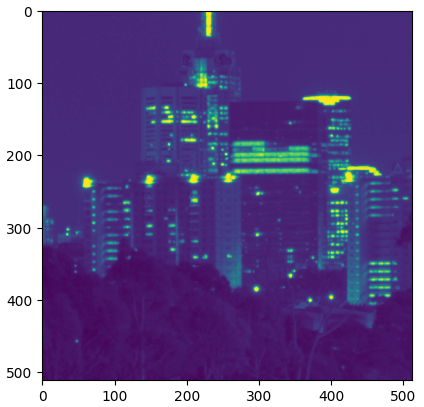
\includegraphics[width=\linewidth]{init.PNG}
                    \caption{Исходное изображение}\label{fig:awesome_image1}
            \end{figure}
        \end{column}
        \begin{column}{0.245\textwidth}
            \begin{figure}
                \centering
                    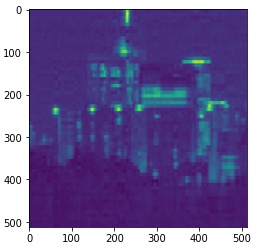
\includegraphics[width=\linewidth]{4.PNG}
                    \caption{96\% сжатие}\label{fig:awesome_image1}
            \end{figure}
        \end{column}
        \begin{column}{0.245\textwidth}
            % \begin{figure}
            %     \centering
            %         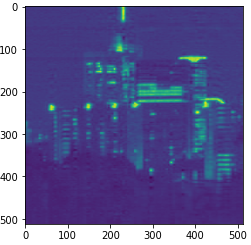
\includegraphics[width=\linewidth]{9.PNG}
            %         \caption{91\% сжатие}\label{fig:awesome_image1}
            % \end{figure}
        \end{column}
        \begin{column}{0.245\textwidth}
            \begin{figure}
                \centering
                    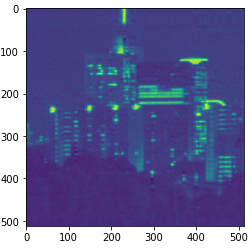
\includegraphics[width=\linewidth]{16.PNG}
                    \caption{84\% сжатие}\label{fig:awesome_image1}
            \end{figure}
        \end{column}
    \end{columns}

\end{frame}

\begin{frame}{Какие были получены результаты?}
    
    \begin{columns}
        \begin{column}{0.47\textwidth}
            \begin{figure}
                \centering
                    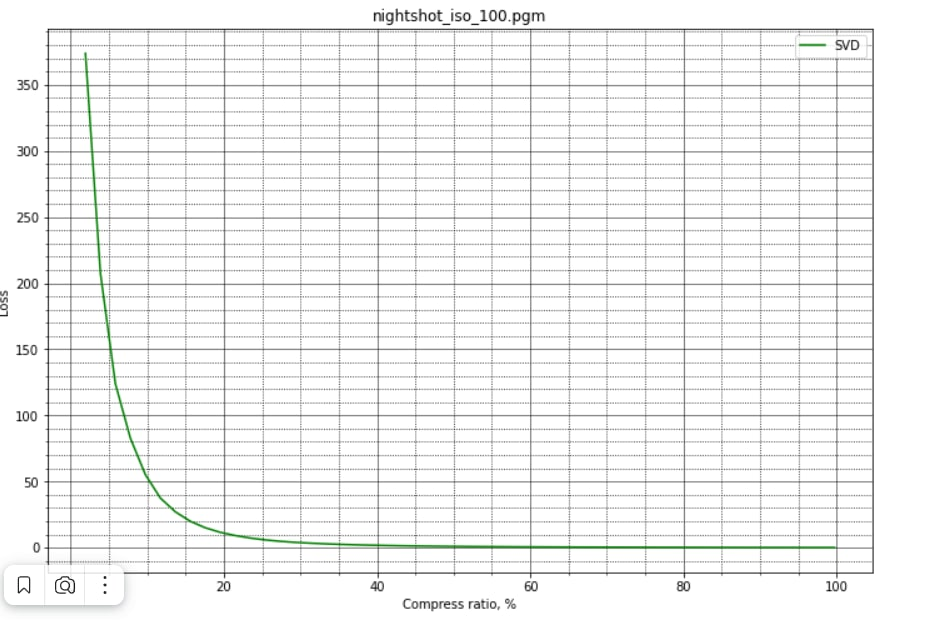
\includegraphics[width=\linewidth]{svd.jpg}
                    \caption{Сжатие SVD}\label{fig:awesome_image1}
            \end{figure}
        \end{column}
        \begin{column}{0.47\textwidth}
            \begin{figure}
                \centering
                    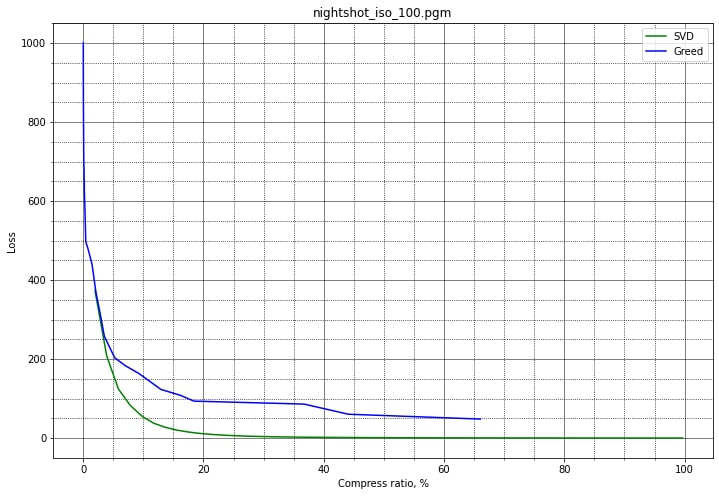
\includegraphics[width=\linewidth]{greed.jpg}
                    \caption{Сжатие алгоритмом из статьи}\label{fig:awesome_image1}
            \end{figure}
        \end{column}
    \end{columns}
        
\end{frame}

\begin{frame}{Что будет дальше?}
\begin{enumerate}
    \item[1)] Освежу в памяти статью \cite{Krumnow2019ComputingEW} 
    \item[2)] Обобщу задачу оптимизации изложенную в статье на тензорные поезда
    \item[3)] Решу полученную задачу
    \item[4)] Проведу численные эксперименты
\end{enumerate}
\end{frame}

\begin{frame}{Источники}
    \bibliographystyle{unsrt}
    \bibliography{biblio}
\end{frame}

\end{document} 


\section{Метрики качества}
\begin{enumerate}
    \item[1)] Относительное сжатие картинок для задачи сжатия
    \item[2)] Относительная ошибка восстановления картинок для задачи восстановления 
    \item[3)] PSNR
    \item[4)] Квадрат нормы Фробениуса разности тензоров
\end{enumerate}

\section{Примерный план}
\begin{itemize}
	\item Для задачи сжатия и восстановления: построить простую тензорную сеть для тензоризированной двумя различными методами картинки, используя  \textit{TT-SVD}, \textit{ALS} и \textit{Adam}.
	\item Проанализировать полученные результаты с помощью объявленных метрик.
	\item Сравнить работу алгоритма сжатия и восстановления с методами, работающими без тензоризации, например: \textit{SVD} и скелетное разложение. 
\end{itemize}
\bibliographystyle{unsrt}
\bibliography{biblio}

\end{document}
